%!TEX root = paper.tex
%%%%%%%%%%%%%%%%%%%%%%%%%%%%%%%%%%%%%%%%%%%%%%%%%%%%%%%%%%%%%%%%%%%%%%%%%%%%%%%%
\section{An End-to-End Lag Model}
\label{sec:model}

The proposed abstract lag model can be adapted to any gaming use case, be it either local, networked, or cloud games. Depending on the specific scenario, more or less components have to be factored in (e.g., the network path and game server with its discrete game ticks for an online game, or the video encoding and decoding elements in cloud gaming). Generally, it derives the \gls{E2E} lag from those factors, specifically including the framerate, tickrate, network \gls{QoS}, client/server messaging rates, and I/O characteristics. The \gls{E2E} lag is here defined to be the time elapsed between the player supplying commands to the input devices and the corresponding audio/video output. Figure~\ref{fig:queuing-model} depicts the overall queuing model.

\begin{figure}[!t]
	\centering
	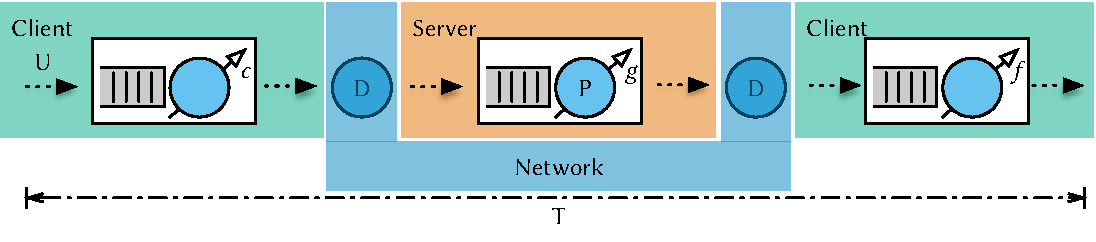
\includegraphics[width=1.0\columnwidth]{../../../models/e2e-lag-model.pdf}
	\caption{Queuing lag model in an online video game case.}
\label{fig:queuing-model}
\end{figure}

To evaluate this model a stochastic \gls{DES} was created\footnote{\url{https://github.com/mas-ude/onlinegame-lag-sim/tree/master/simulation}} and parameterized in a realistic fashion to be representable for each of the three investigated use cases (local, online, cloud). Looking at typical \SI{60}{\hertz} local games (i.e. a frame duration of $\approx \SI{16.6}{\milli\second}$) the median lag is \SIrange{45}{50}{\milli\second}. So even under quasi-optimal circumstances, there is already a considerable amount of \gls{E2E} lag (even without factoring in the delay of the screen and input devices) caused by the interactions of several random and clocked processes. Higher framerates alleviate this somewhat. In the online scenario the framerate has a larger influence on the lag than the tickrate. For low framerates and tickrates, the impact of network delay on the \gls{E2E} lag is almost completely masked. Only if both rates are high enough, the network delay will play a more significant role. This masking effect has large implications for video games and their evaluation. Many evaluations examine the influence of the network delay without considering other contributions to the \gls{E2E} lag. These results indicate that this might not be the best course of action. The effect likely shifts to lower values of the frame- and tickrates when a higher network delay is examined. In the Cloud Gaming scenario in Fig.~\ref{fig:cloud-e2e-delay-sim}, the network delay is set to \SI{40}{\milli\second} (average round-trip); it is seen that the framerate impacts the \gls{E2E} lag more severely than the network does. This result is of particular importance considering how past studies have relied on similarly low framerates as $5-\SI{15}{\hertz}$ when assessing the network influence on cloud gaming. Similarly, our results can provide guidelines for implementors of cloud gaming to factor in the framerate in their calculations accordingly.

\begin{figure}[!t]
	\centering
	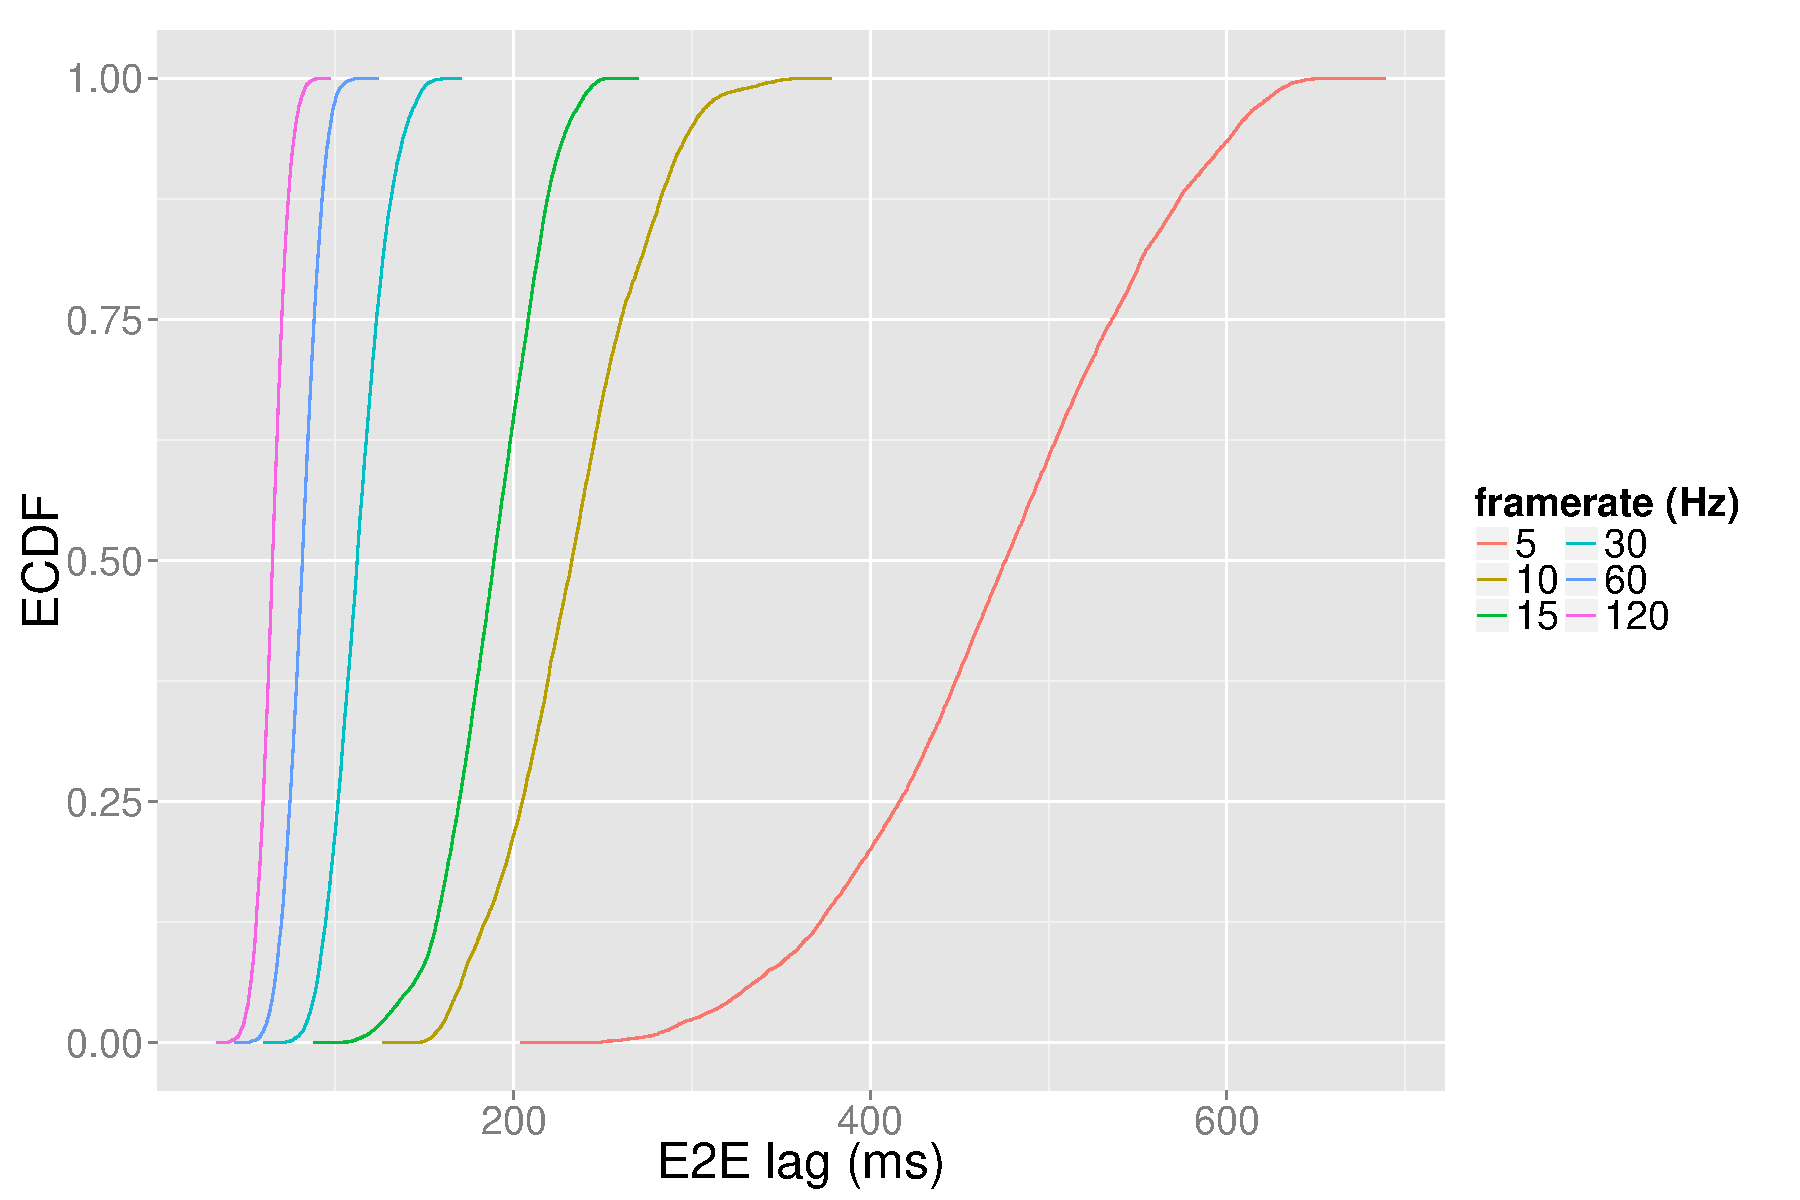
\includegraphics[width=1.0\columnwidth]{../../../simulation/visualization/cloudgaming-lag-cdf.pdf}
	\caption{Influence of the rendering and streaming framerate on the \gls{E2E} lag in the cloud scenario. Vertical intercept denotes the average server, network and codec delay of \SI{68}{\milli\second}.}
\label{fig:cloud-e2e-delay-sim}
\end{figure}


These scenarios reveal the necessity of a tight control over game parameters, such as the framerate, resolution, or input devices, in accordance with the game's type. In order to properly determine this type, novel ways to classify games are needed, as games from the same genre can be vastly different in terms of game speed and necessary reaction times. Better applicable criteria can, e.g., be the \gls{APM}, input accuracy, or the reaction time. A better understanding of these will go a long way in improving the selection of representative games for any evaluation.



% \begin{figure}[!t]
% 	% TODO: adjust the bounding box of the 3dbar plot, instead of playing with fire (aka \vspace)
% 	\centering
% 	\vspace{-6mm}
% 	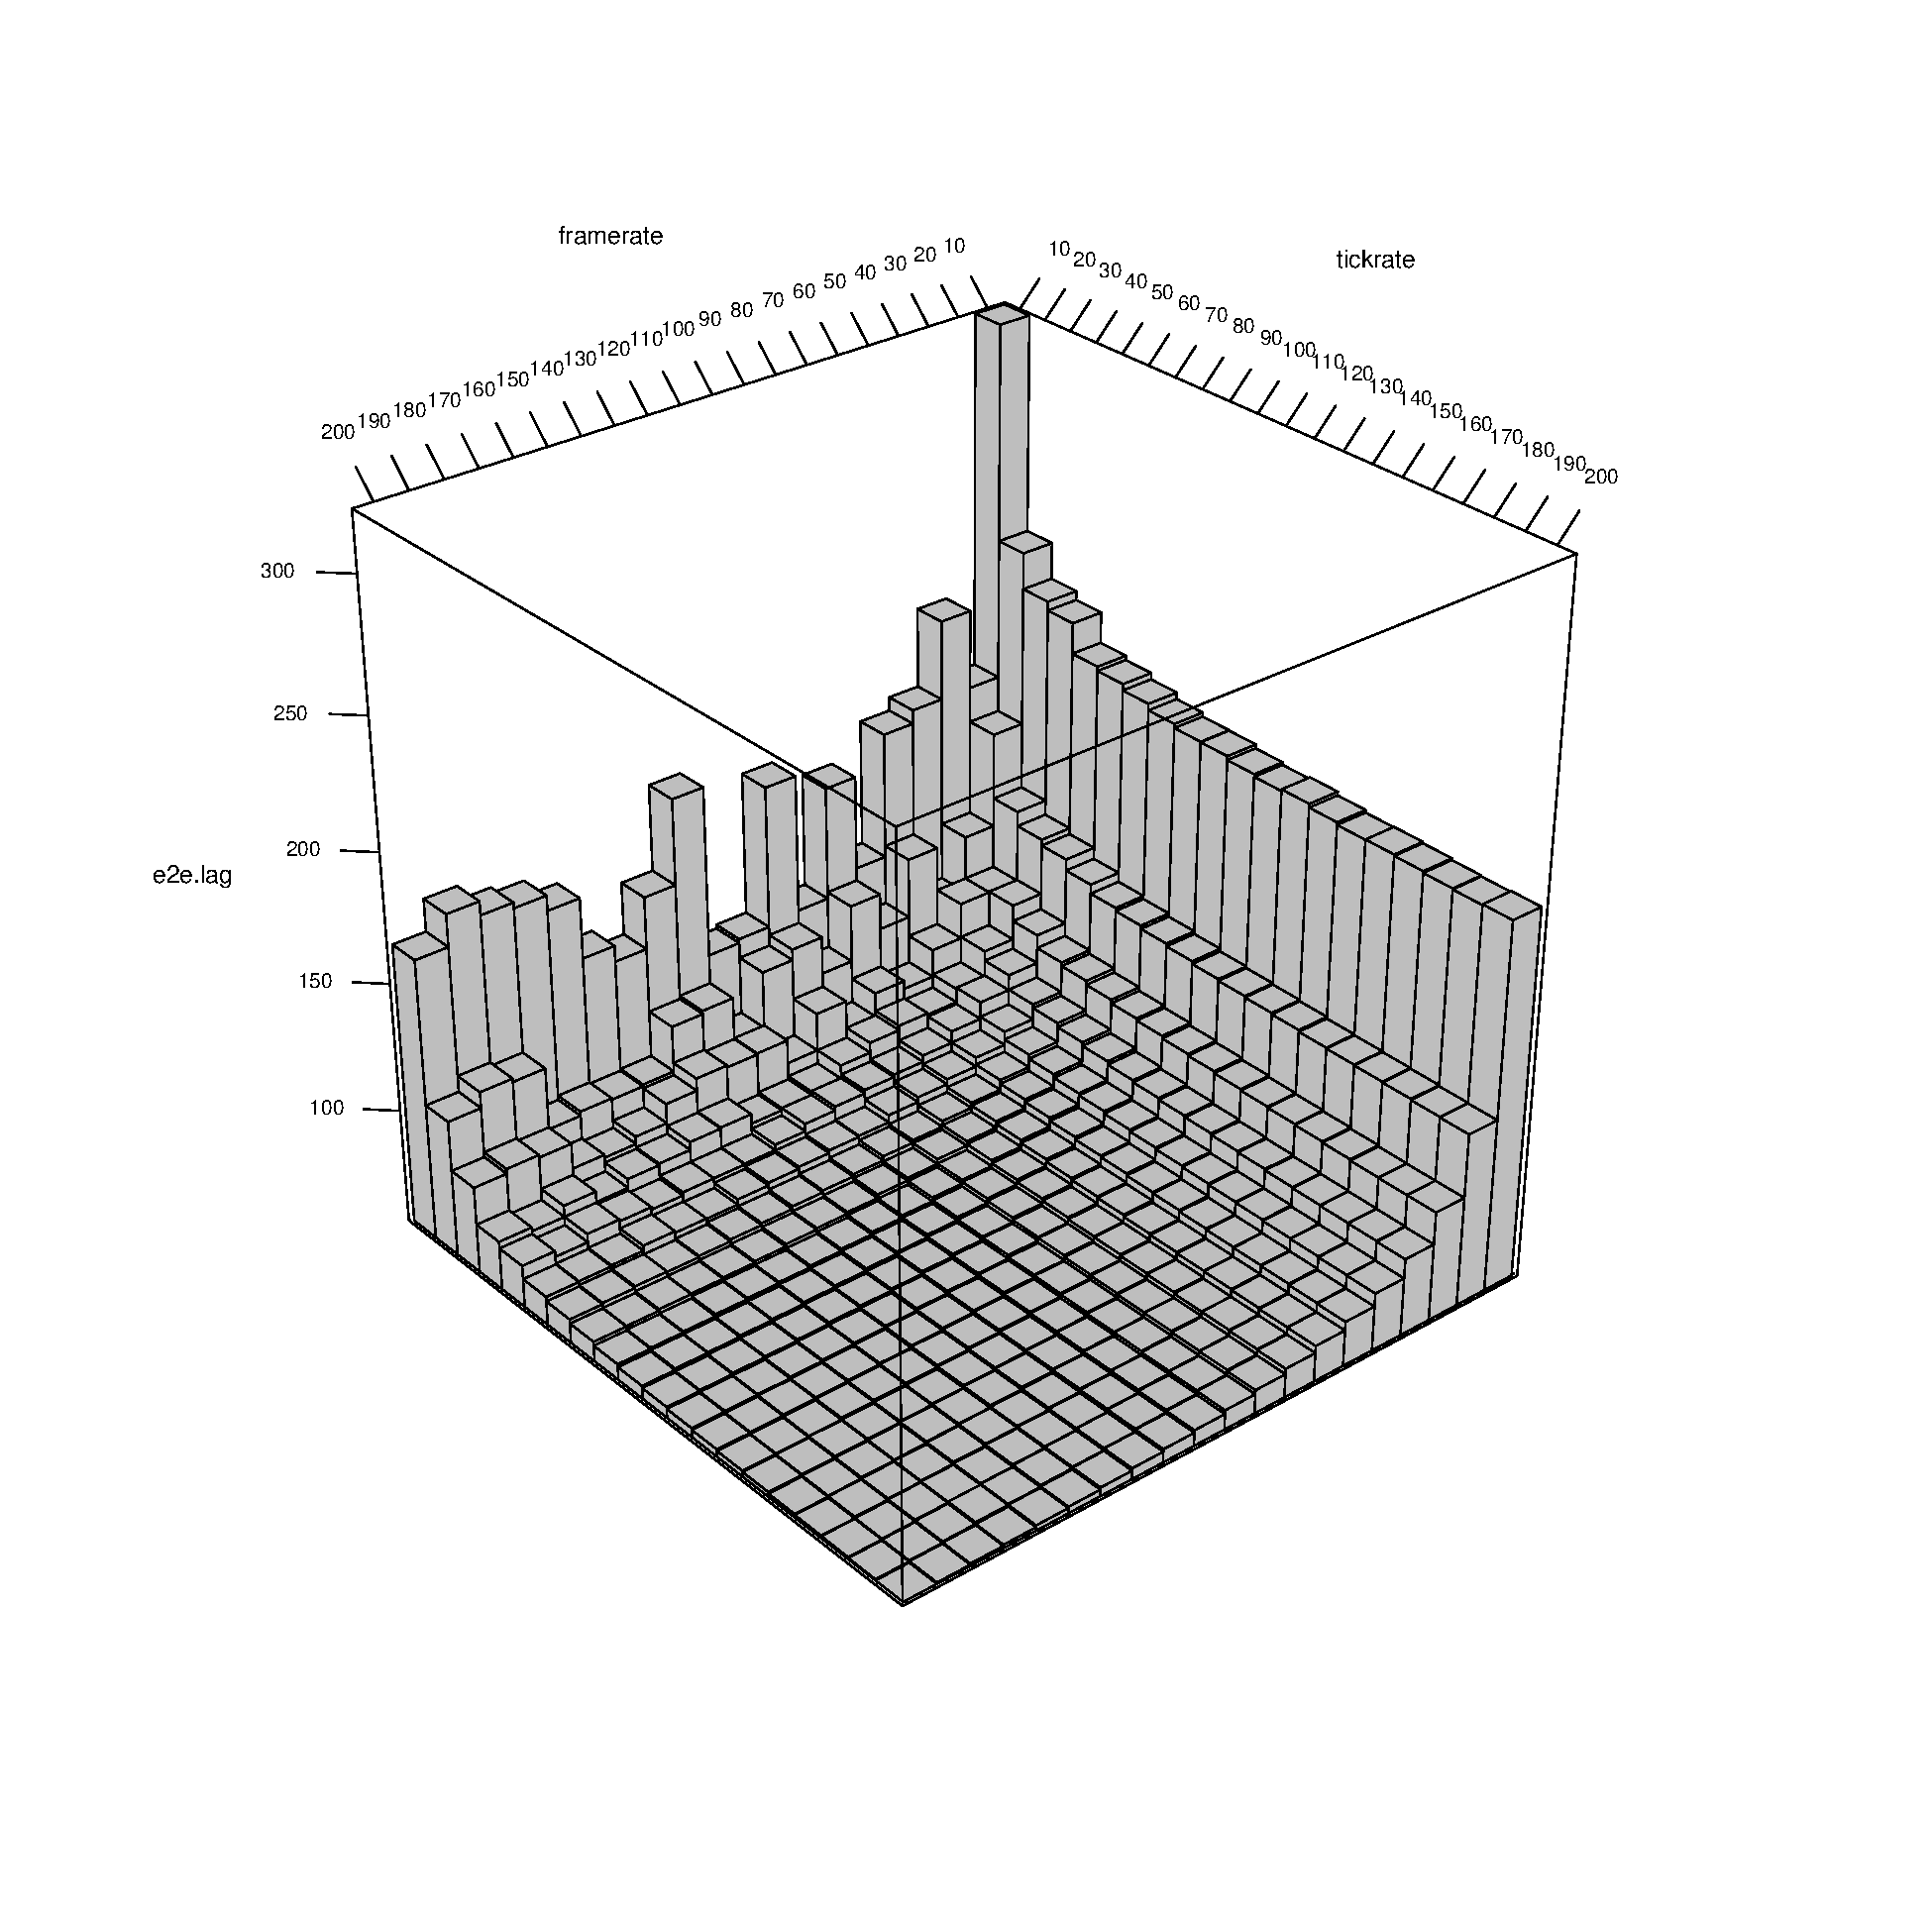
\includegraphics[width=1.0\columnwidth]{../../simulation/visualization/e2e-lag-3dbars.pdf}
% 	\vspace{-15mm}
% 	\caption{Influence of client framerate and server tickrate on the median end-to-end lag in the online game scenario. For high rates $f$, $g$, the lag approaches \SI{43}{\milli\second}.}
% 	% TODO: \hoss{Kann man hier einen stacked bar plot bauen, bei dem man den Networking Anteil sieht? Das wuerde die Aussage gut unterstuetzen.}
% 	% TODO: nicht rechtzeitig für submission deadline, aber für eine nächste version
% \label{fig:3dbars-framerate-tickrate-lag}
% \end{figure}
